\section{Нелінійні рівняння}

\textit{Постановка задачі}. Нехай маємо рівняння $f(x) = 0$, $\overline{x}$ -- його розв’язок, тобто $f (\overline{x}) \equiv 0$. \\

Задача розв‘язання цього рівняння розпадається на етапи:
\begin{enumerate}
	\item Існування та кількість коренів.
	\item Відділення коренів, тобто розбиття числової вісі на інтервали, де знаходиться один корінь.
	\item Обчислення кореня із заданою точністю $\epsilon$.
\end{enumerate}

Для розв'язання перших двох задач використовуються методи математичного аналізу та алгебри, а також графічний метод. Далі розглядаються методи розв'язання третього етапу.

\subsection{Метод ділення навпіл}

Припустимо на $[a, b]$ знаходиться лише один корінь рівняння 
\begin{equation}
	\label{eq:2.1}
	f(x) = 0,
\end{equation}
для $f(x) \in C([a,b])$, який необхідно визначити. Нехай $f(a) \cdot f (b) < 0$. \\

Припустимо, що $f(a) > 0$, $f(b) < 0$. Покладемо $x_1 = \frac{a + b}{2}$ і підрахуємо
$f(x_1)$. Якщо $f_1(x) < 0$, тоді шуканий корінь $x$ знаходиться на інтервалі $(a, x_1)$. Якщо ж $f_1(x) > 0$, то $\overline{x} \in (x_1, b)$, тобто з двох інтервалів $(a, x_1)$ і $(x_1, b)$ вибираємо той, на границях якого функція $f(x)$ має різні знаки, знаходимо точку $x_2$ -- середину вибраного інтервалу, підраховуємо $f(x_2)$ і повторюємо вказаний процес. \\

В результаті отримаємо послідовність інтервалів, що містять шуканий корінь $\overline{x}$, причому довжина кожного послідуючого інтервалу вдвічі менше попереднього. \\

Цей процес продовжується до тих пір, поки довжина отриманого інтервалу $(a_n, b_n)$ не стане меншою за $b_n - a_n < 2 \epsilon$. Тоді $x_{n+1}$, як середина інтервалу $(a_n, b_n)$ пов'язане з $\overline{x}$ нерівністю
\begin{equation}
	\label{eq:2.2}
	|x_n+1 - \overline{x}| < \epsilon.
\end{equation}

Ця умова для деякого $n$ буде виконуватись за теоремою Больцано-Коші. \\

Оскільки
\[ |b_{k + 1} - a_{k + 1} | = \dfrac12 |b_k - a_k|, \]
то
\begin{equation}
	\label{eq:2.3}
	|x_{n+1} - \overline{x}| \le \dfrac{1}{2^{n+1}} (b - a) < \epsilon.
\end{equation}

Звідси отримаємо нерівність для обчислення кількості ітерацій $n$ для виконання умови (\ref{eq:2.2}):
\[ n = n(\epsilon) \ge \left\lfloor \log\left(\dfrac{b-a}{\epsilon}\right) \right\rfloor + 1. \]

Степінь збіжності -- лінійна, тобто геометричної прогресії з знаменником $q = \frac12$. \\

Переваги методу: простота, надійність. Недоліки методу: низька швидкість збіжності; метод не узагальнюється на системи. 

\subsection{Метод простої ітерації}

Спочатку рівняння
\begin{equation}
	\label{eq:2.4}
	f (x) = 0
\end{equation}
замінюється еквівалентним
\begin{equation}
	\label{eq:2.5}
	x = \phi(x)
\end{equation}
Ітераційний процес має вигляді
\begin{equation}
	\label{eq:2.6}
	x_{n+1} = \phi(x_n), \quad n = 0,1,\ldots
\end{equation}

Початкове наближення $x_0$ задається. \\

Для збіжності велике значення має вибір функції $\phi(x)$. Перший спосіб заміни рівняння полягає в відділенні змінної з якогось члена рівняння. Більш продуктивним є перехід від рівняння (\ref{eq:2.4}) до (\ref{eq:2.5}) з функцією $\phi (x) = x + \tau (x) \cdot f (x)$, де $\tau (x)$ -- знакостала функція на тому відрізку, де шукаємо корінь. \\

Кажуть, що ітераційний метод \textit{збігається}, якщо $\Lim_{k\to\infty} x_k = \overline{x}$. \\

Далі $U_r = \{x : |x - a| \le r\}$ відрізок довжини $2r$ з серединою в точці $a$. \\

З'ясуємо умови, при яких збігається метод простої ітерації.

\begin{theorem}
	Якщо $\Max_{x \in U_r} |\phi'(x)| \le q < 1$, то метод простої ітерації збігається і має місце оцінка 
	\begin{equation}
		\label{eq:2.7}
		|x_n - \overline{x}| \le \dfrac{q^n}{1-q}|x_0-x_1| \le \dfrac{q^n}{1-q}(b-a).
	\end{equation}
\end{theorem}

\begin{proof}
	Нехай $x_{k+1}, x_k \in U_r$. Тоді має місце допоміжна нерівність:
	\begin{multline*}
		|x_{k+1} - x_k| = |\phi(x_k) - \phi(x_{k-1})| = |\phi'(\xi_k)(x_k - x_{k-1}) \le (*) \\
		\text{тут }\xi_k = x_k + \theta_k (x_{k+1} - x_k), \quad 0 < \theta_k < 1 \\
		(*) \le |\phi'(\xi_k)| \cdot |x_k - x_{k-1}| \le q |x_k - x_{k-1}| = \ldots = q^k |x_1 - x_0|.
	\end{multline*}
	Використаємо її для доведення теореми:
	\begin{multline}
		\label{eq:2.8}
		|x_{k+p} - x_k| = |x_{k+p} - x_{k+p-1} + \ldots + x_{k+1} - x_k| \le \\
		\le |x_{k+p} - x_{k+p-1}| + \ldots + |x_{k+1} - x_k| \le \\
		\le (q^{k+p-1}+q^{k+p-2}+\ldots+q^k) |x_1 - x_0| = \\
		= \dfrac{q^k - q^{k+p-1}}{1-q}|x_1-x_0| \xrightarrow[k\to\infty]{}0.
	\end{multline}

	Бачимо що $\{x_k\}$ -- фундаментальна послідовність. Значить вона збіжна. При $p\to\infty$ в (\ref{eq:2.8}) отримуємо (\ref{eq:2.7}).
\end{proof}

Визначимо кількість ітерацій для досягнення точності $\epsilon$. З оцінки в теоремі отримаємо \[ |x_n - \overline{x}| \le \dfrac{q^n}{1-q}(b-a) < \epsilon \Rightarrow n(\epsilon) = n \ge \left\lfloor \dfrac{\ln \left(\dfrac{\epsilon (1-q)}{b - a}\right)}{\ln q} \right\rfloor + 1. \]

Практично ітераційний процес зупиняємо при: $|x_n - x_{n-1}| < \epsilon$. Але ця умова не завжди гарантує, що $|x_n - \overline{x}| < \epsilon$.

\begin{remark*}
	Умова збіжності методу може бути замінена на умову Ліпшиця \[|\phi(x) -\phi(y)| \le q \cdot| x - y |,\quad 0 < q < 1.\]
\end{remark*}

Переваги методу: простота; при $q < \frac12$ -- швидше збігається ніж метод ділення навпіл; метод узагальнюється на системи. Недоліки методу: 
\begin{enumerate}
	\item при $q > \frac12$ -- збігається повільніше ніж метод ділення навпіл,
	\item виникають труднощі при зведенні $f (x) = 0$ до $x =\phi (x)$.
\end{enumerate}


\subsection{Метод релаксації}

Якщо в методі простої ітерації для рівняння $x = x +\tau f (x) \equiv\phi (x)$ вибрати $\tau (x) =\tau = \const$, то ітераційний процес приймає вигляд
\begin{equation}
	\label{eq:2.9}
	x_{n+1} = x_n +\tau \cdot f(x_n), \quad n = 0,1,2,\ldots
\end{equation}
$x_0$ -- задано. Метод можна записати у вигляді \[\dfrac{x_{k+1}-x_k}{\tau} = f(x_k), \quad k=0,1,\ldots.\] Оскільки $\phi'(x) =1+\tau\cdot f'(x)$, то метод збігається при умові \[ |\phi'(x)| = |1+\tau \cdot f'(x)| \le q < 1.\]

Нехай $f'(x) < 0$, тоді (\ref{eq:2.7}) запишеться у вигляді: $-q \le 1 +\tau \cdot f'(x) \le q < 1$. Звідси \[\tau \cdot |f'(x_k)| \le 1 + q < 2 \quad \text{і} \quad 0 < \tau < \dfrac{2}{|f'(x)|}. \]

Поставимо задачу знаходження $\tau$, для якого $q = q(\tau) \to \min$. Для того, щоб вибрати оптимальний параметр $\tau$, розглянемо рівняння для похибки $z_k = x_j - \overline{x}$. \\

Підставивши $x_k = x + z_k$ в (\ref{eq:2.9}), отримаємо
\[ z_{k+1} = z_k + \tau \cdot f(\overline{x} + z_k).\]

В припущені $f(x)\in C^{(1)}([a,b])$ з теореми про середнє маємо
\[ f(\overline{x} + z_k) = f(\overline{x}) + z_k \cdot f'(\overline{x} + \theta z_k) = z_k \cdot f'(\overline{x}+\theta z_k) = z_k \cdot f'(\xi_k), \]
\[ z_{k+1} = z_k + \tau \cdot f'(\xi_k) \cdot z_k, \]
\[ |z_{k+1}| \le |1 + \tau \cdot f'(\xi_k)| \cdot |z_k| \le \Max_{\xi_k \in U} |1 + \tau \cdot f'(\xi_k)| \cdot |z_k|, \]
\[ |z_{k+1}| \le \max \{|1-\tau \cdot M_1|, |1-\tau \cdot m_1| \}\cdot |z_k|, \]
\[ m_1 = \Min_{x\in[a,b]} |f'(x)|, \quad M_1 = \Max_{x\in[a,b]} |f'(x)|. \]

Таким чином, задача вибору оптимального параметра зводиться до знаходження $\tau$, для якого функція \[ q(\tau) = \max\{|1-\tau \cdot M_1|,|1-\tau \cdot m_1|\}\]
приймає мінімальне значення: $q(\tau)\to\min$.

\begin{figure}[H]
	\centering
	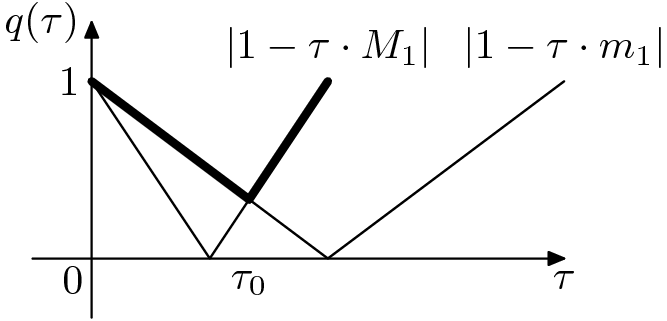
\includegraphics[width=.5\linewidth]{mal-1.png}
\end{figure}

% u:=1cm;
% label.llft(btex $0$ etex, (0,0));
% label.lft(btex $1$ etex, (0,3u/2));
% drawarrow (-u/2,0)--(4u,0);
% drawarrow (0,-u/2)--(0,2u);
% label.lft(btex $q(\tau)$ etex, (0,2u));
% label.bot(btex $\tau$ etex, (4u,0));
% draw (0,3u/2)--(u,0)--(2u,3u/2);
% draw (0,3u/2)--(2u,0)--(4u,3u/2);
% label.top(btex $|1-\tau \cdot M_1|$ etex, (2u,3u/2));
% label.top(btex $|1-\tau \cdot m_1|$ etex, (4u,3u/2));
% draw (4/3u,u/2)--(2u,3u/2) withpen pencircle scaled 2bp;
% draw (0,3u/2)--(4/3u,u/2) withpen pencircle scaled 2bp;
% label.bot(btex $\tau_0$ etex, (4/3u,0));

З графіка видно, що точка мінімуму визначається умовою $|1 - \tau \cdot M_1| = |1 - \tau \cdot m_1|$. \\

Тому
\[ 1 - \tau_0 \cdot m_1 = \tau_0 \cdot M_1 - 1 \Rightarrow \tau_0 = \dfrac{2}{M_1+m_1} < \dfrac{2}{|f'(x)|}.\]

При цьому значенні $\tau$ маємо \[q(\tau_0) = q_0 =\dfrac{M_1-m_1}{M_1+m_1}.\]

Тоді для похибки вірна оцінка \[|x_n-\overline{x}|\le \dfrac{q_0^n\cdot (b-a)}{1-q_0}<\epsilon.\]

Кількість ітерацій \[n = n(\epsilon) \ge \left\lfloor \dfrac{\ln \left(\dfrac{\epsilon\cdot(1-q_0)}{b-a}\right)}{\ln q_0} \right\rfloor + 1.\]	

\begin{problem} 
	Дати геометричну інтерпретацію методу простої ітерації для випадків:
	\[ 0 < \phi'(x) < 1; \quad -1 < \phi'(x) < 0; \quad \phi'(x) < -1; \quad \phi'(x) > 1,\]
\end{problem}

\begin{problem} 
	Знайти оптимальне $\tau = \tau_0$ для методу релаксації при $f'(x) > 0$.
\end{problem}

\subsection{Метод Ньютона (метод дотичних)}

Припустимо, що рівняння $f (x) = 0$ має простий дійсний корінь $\overline{x}$, тобто $f (\overline{x}) = 0$, $f'(\overline{x}) \ne 0$. Нехай виконуються умови: $f (x)\in C^{(1)}([a,b])$, $f (a)\cdot f (b) < 0$. Тоді 
\[0 = f (\overline{x}) = f (x_k + \overline{x} - x_k ) = f (x_k ) + f'(\xi_k ) \cdot (\overline{x} - x_k ),\] 
де $\xi_k=x_k+\theta_k \cdot (\overline{x}-x_k)$, $0 < \theta_k < 1$, $\xi_k \approx x_k$. Тому наступне наближення виберемо з рівняння 
\[ f(x_k) + f'(x_k) \cdot (x_{k+1}-x_k) = 0.\]

Звідси маємо ітераційний процес
\[ x_{k+1} = x_k - \dfrac{f(x_k)}{f'(x_k)}, \quad k = 0,1,2,\ldots, \quad x_0\text{ -- задане}. \]

Метод Ньютона ще називають методом лінеаризації або методом дотичних.

\begin{problem} 
	Дати геометричну інтерпретацію методу Ньютона.
\end{problem}

Метод Ньютона можна інтерпретувати як метод простої ітерації з \[ \phi(x) = x - \dfrac{f(x)}{f'(x)}, \quad \text{тобто} \quad \tau(x) = - \dfrac{1}{f'(x)}. \]

Тому 
\[ \phi'(x) = 1 - \dfrac{f'(x)\cdot f'(x)-f(x)\cdot f''(x)}{(f'(x))^2} = \dfrac{f(x)\cdot f''(x)}{(f'(x))^2}.\]
Якщо $\overline{x}$ -- корінь $f(x)$, то $\phi'(x) = 0$. Тому знайдеться окіл кореня, де \[ |\phi'(x)| = \left|\dfrac{f(x)\cdot f''(x)}{(f'(x))^2}\right|<1.\]

Це означає, що збіжність методу Ньютона залежить від вибору $x_0$. \\

Недолік методу Ньютона: необхідність обчислювати на кожній ітерації не тільки значення функції, а й похідної. \\

Модифікований метод Ньютона позбавлений цього недоліку і має вигляд:
\[ x_{k+1} = x_k - \dfrac{f(x_k)}{f'(x_0)}, \quad k=0,1,2,\ldots. \]

Цей метод має лише лінійну збіжність: $|x_{k+1} - \overline{x}| = O(|x_k-\overline{x}|)$.
\begin{problem} 
	Дати геометричну інтерпретацію модифікованого методу Ньютона.
\end{problem}

В методі Ньютона, для якого $f'(x_k)$ замінюється на $\frac{f(x_k)-f(x_{k-1})}{x_k-x_{k-1}}$ дає метод січних: \[ x_{k+1} = x_k - \dfrac{x_k-x_{k-1}}{f(x_k)-f(x_{k-1})}\cdot f(x_k), \quad k = 1,2,\ldots, \quad x_0,x_1\text{ -- задані}.\]

\begin{problem} 
	Дати геометричну інтерпретацію методу січних.
\end{problem}

\subsection{Збіжність методу Ньютона}

\begin{theorem}
	Нехай $f(x)\in C^{(2)}([a,b])$, $\overline{x}$ -- простий дійсний корінь рівняння
	\begin{equation}
		\label{eq:2.10}
		f (x) = 0
	\end{equation}
	і $f'(x) \ne 0$ при $x\in U_r= \{x: |x -\overline{x}| < r\}$. Якщо
	\begin{equation}
		\label{eq:2.11}
		\dfrac{M_2\cdot|x_0-\overline{x}|}{2m_1} = q < 1
	\end{equation}
	де $m_1 = \Min_{x\in U_r} |f'(x)|$, $M_2 = \Max_{x\in U_r} |f''(x)|$, то для $x_0 \in U_r$ метод Ньютона 
	\begin{equation}
		\label{eq:2.12}
		x_{k+1} = x_k - \dfrac{f(x_k)}{f'(x_k)}
	\end{equation}
	збігається і має місце оцінка
	\begin{equation}
		\label{eq:2.13}
		|x_n - \overline{x}| \le q^{2^n-1} \cdot |x_0 - \overline{x}|.
	\end{equation}
\end{theorem}

\begin{proof}
	З (\ref{eq:2.12}) маємо 
	\begin{equation}
		\label{eq:2.14}
		x_{k+1} - \overline{x} = x_k - \dfrac{f(x_k)}{f'(x_k)} - \overline{x} = \dfrac{(x_k-\overline{x}) \cdot f'(x_k)-f(x_k)}{f'(x_k)} = \dfrac{F(x_k)}{f'(x_k)},
	\end{equation}
	де $F(x) = (x - \overline{x}) \cdot f'(x) - f (x)$, така, що
	\begin{enumerate}
		\item $F(x) = 0$;
		\item $F'(x) = (x - \overline{x}) \cdot f''(x)$;
	\end{enumerate}
	Тоді \[ F(x_k) = F(\overline{x}) + \Int_{\overline{x}}^{x_k}  F'(t) \diff t = \Int_{\overline{x}}^{x_k}  ((t - \overline{x}) \cdot f''(t)) \diff t . \]

	Так як $(t - x)$ не міняє знак на відрізку інтегрування, то скористаємося теоремою про середнє значення:
	\begin{equation}
		\label{eq:2.15}
		F(x_k) = f''(\xi_k) \Int_{\overline{x}}^{x_k}  (t - \overline{x}) \diff t = \dfrac{(x_k-\overline{x})^2}{2} f''(\xi_k),
	\end{equation}
	де $\xi_k = \overline{x} + \theta_k \cdot (x_k - \overline{x})$, $0 <\theta_k < 1$. З (\ref{eq:2.14}), (\ref{eq:2.15}) маємо
	\begin{equation}
		\label{eq:2.16}
		x_{k+1} - \overline{x} = \dfrac{(x_k-\overline{x})^2}{2f'(x_k)} f''(\xi_k).
	\end{equation}
	Доведемо оцінку (\ref{eq:2.12}) за індукцією. Так як $x_0 \in U_r$, то \[|\xi_0 - \overline{x}| = |\theta_0 \cdot (x_0 - \overline{x})| < |\theta_0| \cdot |x_0 - \overline{x}| < r \Rightarrow \xi_0 \in U_r.\]

	Тоді $f''(\xi_0) \le M_2$, тому
	\begin{multline*} 
		|x_1 - \overline{x}| \le \dfrac{(x_0-\overline{x})^2 \cdot M_2}{2m_1} = \dfrac{M_2\cdot|x_0-\overline{x}|}{2m_1}|x_0-\overline{x}| = \\
		= q\cdot |x_0-\overline{x}|=q\cdot |x_0-\overline{x}|<r \Rightarrow x_1\in U_r.
	\end{multline*}

	Ми довели твердження (\ref{eq:2.13}) при $n = 1$. Нехай воно справджується при $n = k$:
	\[ |x_k - \overline{x}| \le q^{2^k-1}\cdot |x_0 - \overline{x}| < r, \quad |\xi_k - \overline{x}| = |\theta_k \cdot (x_k - \overline{x})| < r. \]

	Тоді $x_k, \xi_k \in U_r$. \\

	Доведемо (\ref{eq:2.13}) для $n = k +1$. З (\ref{eq:2.16}) маємо 
	\begin{multline*}
		|x_{k+1}-\overline{x}| \le \dfrac{|x_k - \overline{x}|^2\cdot M_2}{2m_1} \le \left(q^{2^k-1}\right)^2 \dfrac{|x_0-\overline{x}|^2\cdot M_2}{2m_1} = \\
		= q^{2^{k+1}-2} \dfrac{|x_0-\overline{x}|\cdot M_2}{2m_1}|x_0-\overline{x}| = q^{2^{k+1}-1} \cdot |x_0-\overline{x}|.
	\end{multline*}

	Таким чином (\ref{eq:2.13}) справджується для $n = k +1$. Значить (\ref{eq:2.13}) виконується і для довільного $n$. Таким чином $x_n \xrightarrow[n\to\infty]{} \overline{x}$.
\end{proof}

З (\ref{eq:2.13}) маємо оцінку кількості ітерацій для досягнення точності $\epsilon$:
\[ n \ge \left\lfloor\log_2\left(1+\dfrac{\ln \left(\dfrac{\epsilon}{b-a}\right)}{\ln q}\right) \right\rfloor + 1 .\]

Кажуть, що ітераційний метод має \textit{степінь збіжності} $m$, якщо \[ |x_{k+1}-\overline{x}|=O(|x_k-\overline{x}|^m).\]

Для методу Ньютона 
\[|x_{k+1}-\overline{x}| = \dfrac{|x_k-\overline{x}|^2\cdot|f''(\xi_k)|}{2|f'(x_k)|}| \Rightarrow |x_{k+1}-\overline{x}|=O(|x_k-\overline{x}|^2).\]

Значить степінь збіжності методу Ньютона $m=2$. Для методу простої ітерації і ділення навпіл $m=1$.

\begin{theorem}
	Нехай $f(x)\in C^{(2)}([a,b])$ та $\overline{x}$ -- простий корінь рівняння $f (x) = 0$ а також $\forall x\in[a,b]$: $f'(x) \ne 0$. Якщо $f'(x) \cdot f''(x) > 0$ ($f'(x) \cdot f''(x) < 0$) то для методу Ньютона при $x_0 = b$ послідовність наближень $\{x_k \}$ монотонно спадає (монотонно зростає при $x_0 = a$).
\end{theorem}

\begin{problem}
	Довести теорему при 
	\begin{enumerate}
		\item $f'(x) \cdot f''(x) > 0$;
		\item $f'(x) f''(x) < 0$.
	\end{enumerate}
\end{problem}

\begin{problem}
	Знайти степінь збіжності методу січних.
\end{problem}


Якщо $f(a) \cdot f''(a) > 0$ та $f''(x)$ не міняє знак, то потрібно вибирати $x_0 = a$; при цьому $\{x_k \}\uparrow \overline{x}$. \\

Якщо $f(b) \cdot f''(b) > 0$, то $x_0 = b$; маємо $\{x_k \}\downarrow \overline{x}$. Пояснення на рисунку:

% u := 1cm;
% drawarrow (-u/2, 0)--(4u, 0);
% drawarrow (0, -u/2)--(0, 2u);
% draw (u/2,0)--(u/2,u/8);
% draw (7u/2,0)--(7u/2,u/8);
% label.bot(btex $a$ etex, (u/2, 0));
% label.top(btex $b$ etex, (7u/2, u/8));
% draw (u/2,3u/2){dir -75}..(2u,-u/2){dir 0}..(7u/2,-u/4);
% label.top(btex $x_0 = a$ etex, (2u,u));

% u := 1cm;
% drawarrow (-u/2, 0)--(4u, 0);
% drawarrow (0, -u/2)--(0, 2u);
% draw (u/2,0)--(u/2,u/8);
% draw (7u/2,0)--(7u/2,u/8);
% label.top(btex $a$ etex, (u/2, u/8));
% label.bot(btex $b$ etex, (7u/2, 0));
% draw (u/2,-3u/7){dir 75}..(2u,u)..(7u/2,3u/2);
% label.top(btex $x_0 = a$ etex, (2u,3u/2));

\begin{figure}[H]
	\centering
	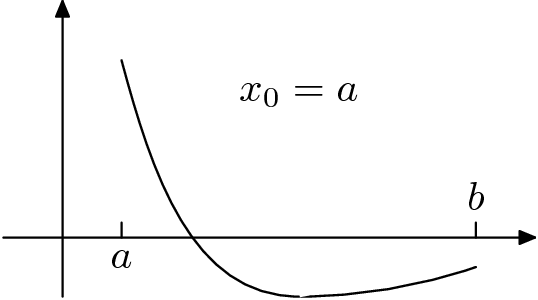
\includegraphics[width=.45\linewidth]{mal-2.png}
	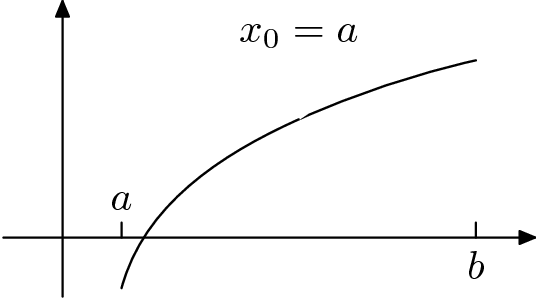
\includegraphics[width=.45\linewidth]{mal-3.png}
\end{figure}

\begin{remark}
	Якщо $\overline{x}$ -- $p$-кратний корінь тобто $f^{(m)} (x) = 0$, $m = \overline{0,p-1}$, $f^{ (p)} (x) \ne 0$, то в методі Ньютона необхідна наступна модифікація \[x_{k+1} = x_k - p\dfrac{f(x_k)}{f'(x_k)} \quad \text{і} \quad q = \dfrac{M_{p+1}\cdot|x_0-\overline{x}|}{m_p \cdot (p+1)}<1.\]
\end{remark}

\begin{remark}
Метод Ньютона можна застосовувати і для обчислення комплексного кореня, тоді ітераційний процес має вигляд \[z_{k+1} = z_k - \dfrac{f(z_k)}{f'(z_k)}, \quad k = 0,1,\ldots.\] В теоремі про збіжність $q = \frac{|z_0-\overline{z}|\cdot M_2}{2m_1}$, де $m_1 = \Min_{z\in U_r} |f'(z)|$, $M_2 = \Max_{z\in U_r} |f''(z)|$. Тут $|z|$ -- модуль комплексного числа $z$.
\end{remark}

Переваги методу Ньютона: 
\begin{enumerate}
\item висока швидкість збіжності;
\item узагальнюється на системи рівнянь; 
\item узагальнюється на комплексні корені.
\end{enumerate}
Недоліки методу Ньютона: 
\begin{enumerate}
	\item на кожній ітерації обчислюється не тільки $f (x_k )$ , а і похідна $f'(x_k)$;
	\item  збіжність залежить від початкового наближення $x_0$, так як від нього залежить умова збіжності $q = \frac{M_2\cdot |x_0-\overline{x}|}{2m_1} < 1$;
	\item потрібно, щоб $f (x)\in C^{(2)}([a,b])$.
\end{enumerate}